%!TEX root = main.tex
\section{Einführung}
		
	\begin{minipage}[t][\textheight][t]{0.76\textwidth}

	Diese Arbeit beschäftigt sich mit der Verallgemeinerung von Knoten- und Verschlingungsinvarianten. Das Ziel ist die Ausarbeitung des Beweises von McMullens Ungleichung (2002) der Alexander-Norm und der Thurston-Norm die aus 3-Mannigfaltigkeiten hervorgehen. Der Kontext der 3-Mannigfaltigkeiten beinhaltet große Teile der Knoten- und Verschlingungstheorie  --- in diesem Sinne verallgemeinert man das Alexander-Polynom und das Geschlecht einer Verschlingung.

	Die Theorie der Knoten beschäftigt sich mit Äquivalenzklassen von Knoten und dem Finden von Invarianten solcher Äquivalenzklassen. In der differenzierbaren Kategorie bezeichnet man mit einem Knoten eine glatte orientierte Einbettung $S^1\into S^3$ und man definiert zwei Knoten als äquivalent, wenn ein orientierungserhaltener Diffeomorphismus $S^3\to S^3$ existiert, der beide Knoten ineinander überführt. Insbesondere entstehen in der differenzierbaren Kategorie keine exotischen Exemplare eines Knotens, die man als "`wild"' bezeichnet. Als häufig betrachtete Invariante hat sich die orientierte Diffeomorphieklasse der kompakten 3-Mannigfaltigkeit ergeben, die man das Knotenkomplement nennt. Dieses entsteht durch Entnehmen einer offenen Tubenumgebung des eingebetteten Knotens $S^1 \into S^3$ und ist eine naheliegende Knoteninvariante. Letzteres bedeutet: Äquivalente Knoten haben diffeomorphe Knotenkomplemente durch einen orientierungserhaltenden Diffeomorphismus. Häufig stellen sich Knoteninvarianten lediglich als Invarianten der Knotenkomplemente heraus; etwa bezeichnet man mit der Gruppe eines Knotens die Fundamentalgruppe des Komplements. Um die Qualität und Feinheit dieser aus dem Komplement entstehenden Invarianten zu beurteilen, ist es zunächst wichtig jene des Knotenkomplements zu beurteilen. Es gibt unzählige Ergebnisse, die aus Berechnungen auf dem Knotenkomplement entstehen, woraus sich die Relevanz der Frage ableitet. 1989 zeigen Gordon und Luecke~\cite{Gordon.1989} die Umkehrung, dass orientiert diffeomorphe 3-Mannigfaltigkeiten die aus Knotenkomplementen entstehen, aus äquivalenten Knoten entstehen. Es handelt sich bei dem Knotenkomplement also um eine vollständige Knoteninvariante. Um Invarianten die aus dem Knotenkomplement entstehen, soll es in dieser Arbeit gehen.


	\vfill
	\begin{minipage}[t]{0.7\textwidth}
		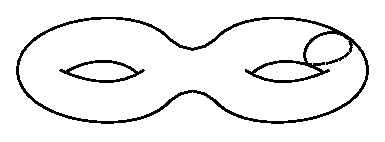
\includegraphics{zyklbott} 
	\end{minipage}
	\begin{minipage}[t]{0.2\textwidth}
	\vspace{-1cm}
	\huge$\longleftarrow$
	\vfill

	\end{minipage}
	\vspace{.63cm}
		\captionof{figure}{Unendlich zyklische Überlagerung} \label{fig:zykl}
	\end{minipage}
	\hfill
	\begin{minipage}[t]{0.2\textwidth}
	\vfill \begin{flushright}
		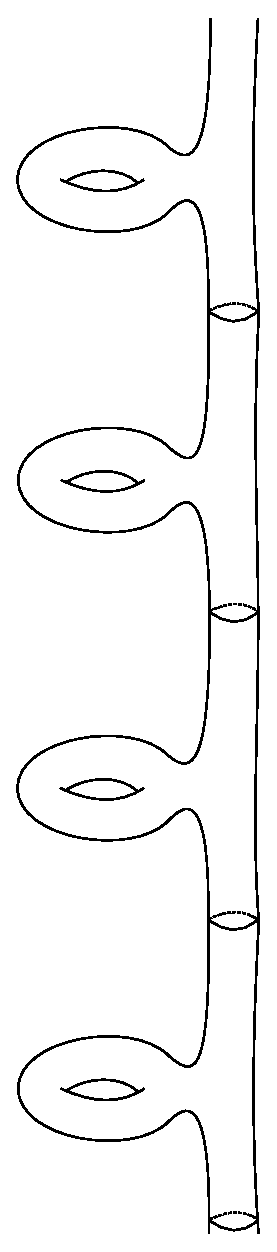
\includegraphics{zyklright} 
	\end{flushright}
	\end{minipage}

	Alexander definiert 1928 eine topologische Invariante des Knotenkomplements (vgl.\,\cite{Alexander.1928}), die einem Knotenkomplement eine Klasse von Laurentpolynomen mit eindeutigem Grad zuordnet. 1934 stellt Seifert in seiner Arbeit "`Geschlecht von Knoten"'~\cite{Seifert.1934} mit dem Knotengeschlecht eine Invariante vor, welche die minimale Komplexität einer orientierten eingebetteten Fläche berechnet, die den Knoten aufspannt (nach der Klassifikation von Flächen wird diese in Termen des Geschlechts gemessen) und gibt eine explizite Konstruktion für die Existenz solcher Flächen an. Dieses Knotengeschlecht liefert die Möglichkeit jeden Knoten von dem Unknoten zu unterscheiden. Das bedeutet, dass nur nur der Unknoten aus dem Rand einer eingebetteten Scheibe hervorgeht. Natürlich liefert die sogennante Seifert-Konstruktion, mit der Seifert die Existenz solcher Flächen gezeigt hat, eine Fläche mit Geschlecht. Es ist jedoch ein deutlich komplizierteres Unterfangen, wenn man zeigen möchte, dass eine gefundene Fläche in ihrer Komplexität nicht unterboten werden kann. Entsprechend günstig erweist sich Seiferts Resultat, dass der Grad des Alexander-Polynoms eines Knotens eine untere Schranke für sein Geschlecht definiert. Hat man also eine eingebettete orientierte Fläche gefunden, deren Rand ein Knoten ist, von der man vermutet minimales Geschlecht zu haben, so kann man den Grad des Alexander-Polynoms berechnen und verifiziert in manchen Fällen die Vermutung.

	Der wesentliche Gegenstand dieser Arbeit ist die Verallgemeinerung dieser auf Knotenkomplementen definierten Invarianten zu Invarianten auf kompakten orientierbaren 3-Mannigfaltigkeiten mit Rand, der maximal aus Tori besteht. Für diese Invarianten stellt McMullen~\cite{MCMULLEN.2002} fest, dass sich auch die oben erwähnte Abschätzung aus der Knotentheorie verallgemeinern lässt. Diese Arbeit beschäftigt sich mit genau diesem Resultat, welches dieser Arbeit als Haupttheorem~\ref{thm:haupttheorem} zugrunde liegt.

	Um dem Leser den Einstieg in die Arbeit möglichst angenehm zu gestalten, sei im Folgenden noch die Art der Verallgemeinerungen und der Aufbau der Arbeit skizziert.

    Im Falle eines Knotens berechnet sich die erste Kohomologie des Komplementes zu einer freien abelschen Gruppe von Rang 1. Die orientierte Seifert-Fläche (welche den Knoten aufspannt) lässt sich als Homologieklasse auffassen, vgl.\,Bemerkung~\ref{bem:untermannigfaltigkeitenalshomologie}. Als solche ist sie Lefschetz dual zu einem $\phi$ der ersten Kohomologie. Nun kann man die folgenden --- etwas verkomplizierenderen --- Formulierungen für die Knoteninvarianten betrachten, die den Zusammenhang mit den Verallgemeinerungen darstellen. Die Alexander-Norm von $\phi$ wertet den Grad des Alexander-Polynoms des Knoten aus, vgl.\,Kapitel~\ref{sec:links}. Für allgemeinere 3-Mannigfaltigkeiten, ordnet sie Kohomologieklassen ähnliche Auswertungen an. Und die Thurston-Norm einer Kohomologieklasse verallgemeinert die minimale Komplexität aller dualen, orientierten, eingebetteten Flächen. Im Falle eines Knotens würde sich diese aus einer geschlechtsminimierende Seifert-Fläche berechnen.

    Es stellt sich heraus, dass alle betrachteten Invarianten eine enge Beziehung zu unendlich zyklischen Überlagerungen haben. Diese können etwa durch Aufschneiden und Verkleben an einer zusammenhängenden 1-kodimensionalen Untermannigfaltigkeit gewonnen werden, siehe zum Beipsiel Abbildung~\ref{fig:zykl}. Diese Abbildung ist für die Intuition und das Verständnis erheblich --- man könnte dem Leser fast raten, vor und nach jedem Kapitel die Abbildung~\ref{fig:zykl} zu betrachten und immer wieder neu zu reflektieren.

    Der Aufbau der Arbeit lässt sich wie folgt beschreiben: Das erste Kapitel bereitet das nötige algebraische und topologische Werkzeug für die Definitionen und Berechnungen der verallgemeinerten Invarianten vor. Weiter beschreibt es Konstruktionen, die in späteren Beweisen zielführend sein werden. Das nächste Kapitel definiert die Thurston-Norm der Mannigfaltigkeit $M$ eines Elementes von $\phi \in H^1(M;\ZZ)$ und beweist eine Abschätzung gegen $b_1(\ker\phi)$. Anschließend präsentiert das Kapitel~\ref{sec:alexdefs} die Alexander-Norm und widmet dieser eine ausführliche algebraische Betrachtung. Weiter stellt es einen Zusammenhang der Alexander-Norm mit $b_1(\ker\phi)$ her. Diese Ergebnisse liefern den Beweis des Theorems, der mit einer Reihe von Modifikationen und Ergänzungen an die Beweisführung aus~\cite{MCMULLEN.2002} angelehnt ist. Das letzte Kapitel stellt weiterführende Fragen und gibt einige Anwendungen und Beispiele für Berechnungen an.   

    Bevor nun das Haupttheorem der Arbeit angegeben wird, möchte ich mich ausdrücklich bei meiner Betreuerin Prof. Ursula Hamenstädt bedanken. Nicht nur für die Wahl des interessanten Themas, sondern vor allem auch für die qualitative Betreuung und den hohen Zeit- und Geduldaufwand, den sie dafür eingebracht hat. Die gemeinsamen Diskussionen hatten eine extrem hohe Lerndichte für mich und das Wissen, dass ich im Rahmen der Bachelorarbeit gewonnen habe, geht weit über das Niedergeschriebene hinaus. Weiter möchte ich Prof. Matthias Kreck danken, dessen exzellente Vorlesung über die Differentialtopologie meine Intuition und Geschicklichkeit in differentialtopologischen Betrachtungen geprägt hat und mir einen guten Einstieg in die Bachelorarbeit ermöglicht hat.
    %in diesem Rahmen?

    \begin{thm}[McMullen]
    \label{thm:haupttheorem}
    	Sei $M$ eine kompakte, zusammenhängende, orientierbare Mannigfaltigkeit der Dimension 3. Falls der Rand dieser Mannigfaltigkeit nicht leer ist, so soll er aus einer Kollektion von Tori bestehen. Dann gilt folgende Abschätzung für die Alexander-Norm und die Thurston-Norm $\alex \cdot ,\thur \cdot : H^1(M;\ZZ) \to \RR$ der 3-Mannigfaltigkeit:
    	\[
    		\alex \phi \leq 
    		\begin{cases}
    			\thur \phi + 1+ b_3(M) &\text{, falls } b_1(M)\leq 1 \text{ und } \phi: \pi_1(M) \onto \ZZ \\
    			\thur \phi &
    		\end{cases}
    	\]
    	Entsteht $\phi$ als Rückziehung einer Faserung $M\to S^1$, so gilt Gleichheit.
    \end{thm}